\section{Raytracing}

\subsection{Farbwahrnehmung und Farbmodelle}
\subsection{Globale Beleuchtungsmodelle und Rendergleichung}
\subsubsection{Photometrie}
Die Radiantenergie $Q$ ist die Lichtenergie. Sie wird durch einen Strom von Photonen erzeugt. Die Energie eines Photons ist 
durch $E=h \cdot f$ geben, wobei $h$ das konstante Planksche Wirkungsquantum und $f$ die Frequenz der Welle ist (Welle-Teilchen Dualismus).  
Die Ableitung nach der Zeit
\begin{align}
\phi := \frac{\partial Q}{\partial t}
\end{align}
wird als Radiant Flux oder Strahlungsleistung bezeichnet. Diese  beschreibt den Energiefluss, beziehungsweise den Energie-Eintritt und Energie-Austritt.

Der Radiant Flux in einem infinitesimal dünnen Strahl vom Punkt $x$ in Richtung $\omega$ wird als Radiance $L(x, \omega)$ bezeichnet was  Formal durch
\begin{align}
L(x, \omega) := \frac{d^2 \phi}{\cos(\theta) dA \cdot d\omega}
\end{align}
ausgedrückt wird. Die Radiance ist also der Radiant Flux pro infinitesimale Flächeneinheit $\cos(\theta) dA$ und pro  Raumwinkel $d \omega$.
\subsubsection{BRDF und Reflectancegleichung }
Die sogenannte bidirektionale Reflektanzverteilungsfunktion (engl. Bidirectional Reflectance Distribution Function, BRDF)
ist eine Funktion $f_r (x, \omega_i, \omega_r)$, die das Reflexionsverhalten der Oberfläche eines Materials beschreibt. 
Sie hat als Eingabe die ausgehende Richtung $\omega_r$ und die eingehende Richtung  $\omega_i$ am Punkt $x$. 
Sie  liefert den Quotienten aus Strahlungsdichte und Bestrahlungsstärke für die ausgehende Richtung $\omega_r$ und die eingehende Richtung  $\omega_i$ am Punkt $x$.
Sie gibt somit die Abhängigkeit des reflektierten Lichts von der einfallenden Lichtstärke an: 
\begin{align}
dL_r = f_r(x, \omega_i, \omega_r) dE =   f_r(x, \omega_i, \omega_r) L_i(x,\omega_i) \cos(\theta_i) d \omega_i\\
L_r(x, \omega_r) = \int_{H^2} dL_r =    \int_{H^2}f_r (x, \omega_i, \omega_r) \cdot L(x, \omega_i) \cos(\theta_i) d\omega_i
\end{align}
Letztere Gleichung wird auch Reflectance-Gleichung genannt.
 \begin{figure}[H]
    \centering
    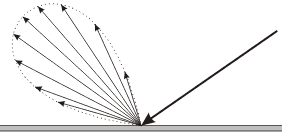
\includegraphics[width=0.6\textwidth]{images/brdf2.png}
    \caption{BRDF Funktion}
    \label{fig:raytracin_brdf}
\end{figure}

\subsubsection{Das photometrische Grundgesetz}
 
\subsubsection{Die Rendergleichung (Erste und zweite Form)}

\subsection{Raycasting}
\subsubsection{"Klassisches" Raytracing}
\subsection{Radiocity Verfahren}
\subsubsection{Monte Carlo Integration und Pathtracing}
\subsubsection{Raymarching}
\subsubsection{Klassifikation der Verfahren}

\subsubsection{Datenstrukturen für Bereichsabfragen}


\subsection{Labor}
\subsubsection{Blender}
\subsubsection{Echtzeitfähiges Raymarching in WebGL}
